% Chapitre 3 — Méthodologie (version française)

\chapter{Méthodologie}

\begin{quote}
\textbf{Note sur les sources.} Ce chapitre décrit la méthodologie technique de la campagne de mesure. Les sources bibliographiques sont citées lorsque la méthodologie est directement inspirée ou adaptée de travaux antérieurs. Les choix d'ingénierie logicielle généraux (utilisation d'API, paramètres de format de données, tests statistiques) ne sont pas attribués à des sources.
\end{quote}
\bigskip
\section{Vue d'ensemble}
\label{sec:3.1}

\subsection{Objectif méthodologique}
\label{subsec:3.1.1}

L'objectif méthodologique central de ce mémoire est de capturer la \textbf{diversité géographique et temporelle des réponses DNS} pour un corpus représentatif de domaines populaires, à l'aide de mesures actives géographiquement distribuées, de manière reproductible, éthiquement rigoureuse et réalisable dans le budget de ressources disponible. Le système doit répondre à quatre questions de recherche empiriques :

\begin{itemize}
  \item \textbf{Q1} : Quelle proportion des domaines les mieux classés dans Tranco retourne des réponses DNS géographiquement différenciées, et quels mécanismes d'infrastructure expliquent la différenciation ?
  \item \textbf{Q2} : Quelle est la stabilité temporelle des réponses DNS pour les domaines populaires aux échelles jour, semaine et mois ?
  \item \textbf{Q3} : Les biais géographiques de la distribution des sondes RIPE Atlas limitent-ils significativement la capacité à observer la variation DNS géographique ?
  \item \textbf{Q4} : Quel est l'impact mesurable du type de résolveur --- résolveur ISP local versus service DNS public --- sur les réponses DNS observées ?
\end{itemize}

\subsection{Architecture du système}
\label{subsec:3.1.2}

Le système de mesure est organisé en cinq étapes séquentielles, inspirées de l'architecture d'OpenINTEL~\cite{vanRijswijk2016} mais adaptées aux contraintes et capacités de la plateforme RIPE Atlas :

\begin{enumerate}
  \item \textbf{Préparation du corpus de domaines} : Récupération et filtrage de la liste Tranco Top 10\,000.
  \item \textbf{Planification des mesures} : Configuration et déploiement des campagnes de mesure DNS RIPE Atlas.
  \item \textbf{Collecte de données} : Récupération automatique quotidienne des résultats via l'API REST RIPE Atlas.
  \item \textbf{Stockage et prétraitement} : Analyse syntaxique, validation et archivage au format Avro/Parquet.
  \item \textbf{Analyse} : Analyse quantitative répondant à Q1--Q4.
\end{enumerate}

Le compromis de conception central est la tension à trois dimensions entre la \textbf{couverture de domaines} (combien de domaines mesurer), la \textbf{couverture géographique} (combien de sondes distribuées géographiquement) et la \textbf{résolution temporelle} (fréquence de mesure), le tout borné par le budget limité en crédits RIPE Atlas. La configuration décrite dans ce chapitre cible 10\,000 domaines $\times$ 100 sondes $\times$ une fois par jour comme point de fonctionnement principal, avec une campagne supplémentaire de comparaison de résolveurs pour Q4. La figure~\ref{fig:pipeline_collecte} présente l'architecture du pipeline en cinq étapes.

\begin{figure}[tp]
  \centering
  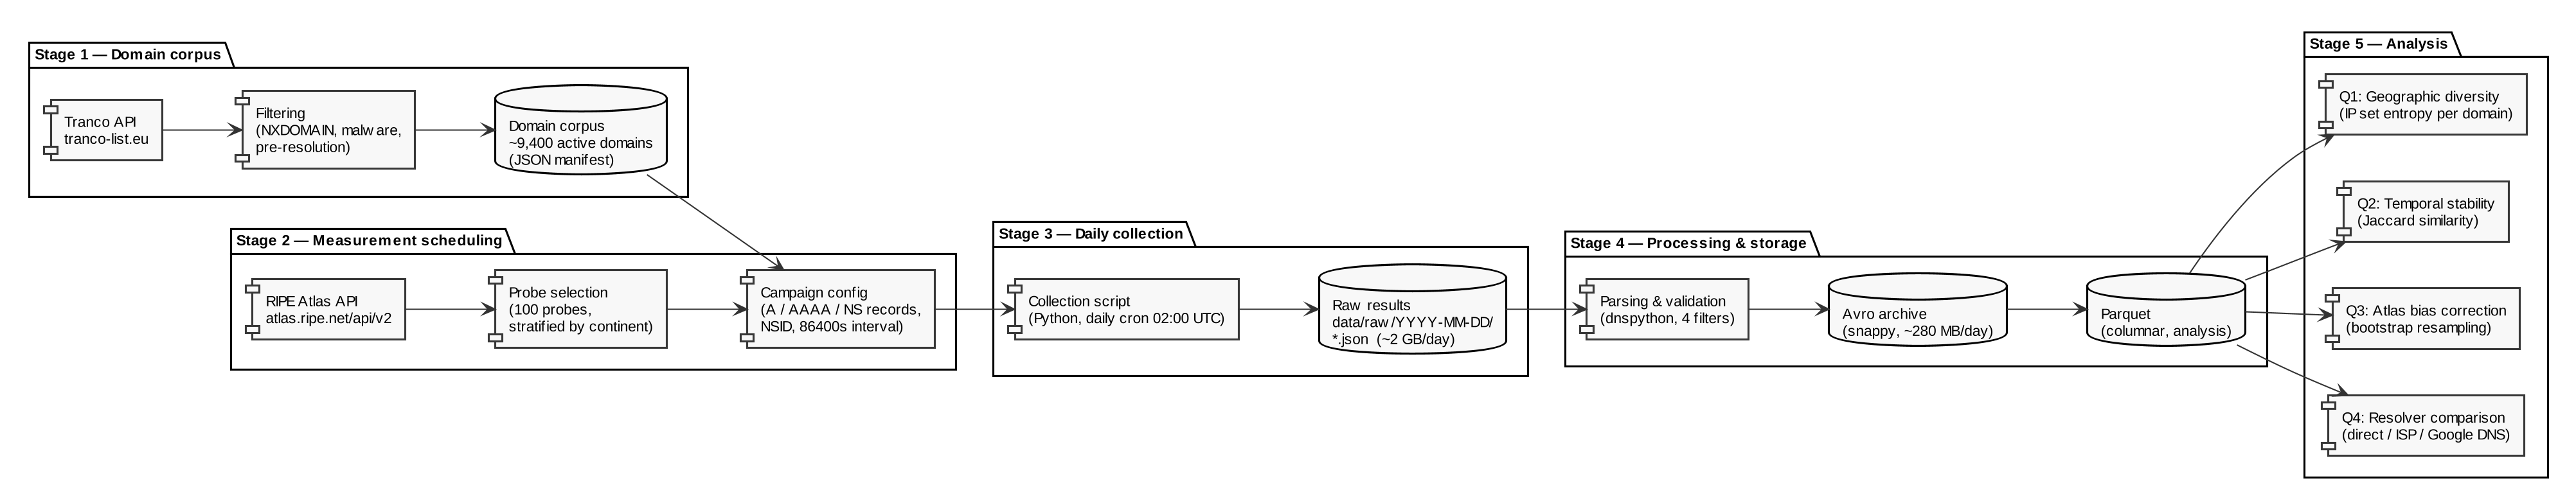
\includegraphics[width=\linewidth]{figures/fig7_pipeline_collecte.png}
  \caption{Architecture du pipeline de mesure en cinq étapes. L'étape~1 prépare le corpus de domaines à partir de l'API Tranco. L'étape~2 planifie les campagnes RIPE Atlas à partir d'un ensemble de sondes stratifié. L'étape~3 collecte les résultats JSON bruts quotidiennement. L'étape~4 analyse syntaxiquement, valide et archive au format Avro/Parquet. L'étape~5 effectue l'analyse quantitative pour les questions de recherche Q1--Q4.}
  \label{fig:pipeline_collecte}
\end{figure}

\bigskip
\section{Sélection du corpus de domaines}
\label{sec:3.2}

\subsection{Configuration de la liste Tranco}
\label{subsec:3.2.1}

Le corpus de domaines est la liste \textbf{Tranco Top 10\,000}, récupérée via l'API Tranco. Le choix de Tranco plutôt que les listes commerciales (Alexa, Cisco Umbrella, Majestic) est motivé au chapitre~2 (section~2.6) et repose sur trois propriétés établies par Le Pochat et al.~\cite{LePochat2019} : stabilité (0,6\,\% de changement quotidien contre environ 50\,\% pour Alexa post-2018), résistance à la manipulation (effort de manipulation quadruplé par rapport aux listes à source unique), et archivabilité (chaque liste générée se voit attribuer un identifiant unique récupérable indéfiniment via un permalien).

La liste Tranco est générée avec la configuration fixe suivante pour garantir la reproductibilité :

\begin{verbatim}
Taille de la liste :     10 000 domaines
Fenêtre de moyennage :   30 jours (défaut Tranco)
Méthode d'agrégation :   règle de Dowdall (pondère le rang par 1/rang_i par source)
Sources :                Alexa, Cisco Umbrella, Majestic, Quantcast
Filtres :                réactivité (HTTP 200), navigation sécurisée (Google Safe Browsing API)
\end{verbatim}

La règle de Dowdall a été choisie plutôt que le comptage Borda car sa pondération 1/rang reflète mieux la distribution Zipf du trafic Internet : la différence entre les rangs 1 et 2 est traitée comme plus significative que la différence entre les rangs 999 et 1\,000.

La liste est \textbf{mise à jour hebdomadairement} (chaque lundi) pour capturer l'évolution lente du corpus de domaines populaires tout en limitant le taux de changement induit par les mises à jour. Le taux de changement quotidien stable de 0,6\,\% de Tranco~\cite{LePochat2019} signifie que même les mises à jour hebdomadaires produisent un renouvellement minimal de l'ensemble de domaines. Chaque mise à jour hebdomadaire enregistre l'identifiant exact de la liste Tranco utilisée, l'horodatage de génération, et le delta des domaines ajoutés et supprimés par rapport à la liste de la semaine précédente. Les domaines qui quittent le Top 10K pendant la campagne de mesure sont conservés en mesure active deux semaines supplémentaires pour capturer tout comportement DNS de transition.

\subsection{Taille du corpus de domaines}
\label{subsec:3.2.2}

Le choix de 10\,000 domaines équilibre trois exigences concurrentes :

\textbf{Représentativité} : Le Tranco Top 10K contient les domaines responsables de la grande majorité du trafic web mondial, incluant les grands services CDN (plateformes de streaming, moteurs de recherche, réseaux sociaux, fournisseurs cloud) qui sont censés présenter la plus riche variation DNS géographique.

\textbf{Faisabilité} : Avec 100 sondes par mesure, un type de mesure (enregistrement A) et une mesure par domaine par jour, le corpus Top 10K génère environ un million de résultats de mesure par jour. Ce volume est gérable dans le budget de crédits RIPE Atlas disponible. Le Top 100K serait un ordre de grandeur plus grand et nécessiterait substantiellement plus de crédits.

\textbf{Précédent établi} : Le Tranco Top 10K est la taille de corpus standard utilisée dans les études de mesure DNS et web~\cite{Calder2015,Wang2018}, permettant une comparaison directe avec les travaux antérieurs.

\subsection{Filtrage des domaines}
\label{subsec:3.2.3}

Avant le début de la campagne de mesure, chaque domaine de la liste Tranco Top 10K est pré-validé en trois étapes :

\textbf{Validité technique} : Une requête DNS d'enregistrement A est émise depuis l'infrastructure de mesure locale. Les domaines retournant \texttt{NXDOMAIN} ou \texttt{SERVFAIL} --- indiquant des domaines non enregistrés ou défectueux --- sont exclus. Les domaines sans enregistrement A sont exclus des mesures d'enregistrement A mais conservés dans l'ensemble de mesure d'enregistrement NS.

\textbf{Filtrage de sécurité} : Les domaines signalés par l'API Google Safe Browsing comme hébergeant des logiciels malveillants, du phishing ou des logiciels indésirables sont exclus. Ce filtre protège à la fois les hôtes de sondes et l'intégrité du corpus en tant que référence pour l'infrastructure Internet légitime.

\textbf{Pré-résolution des serveurs faisant autorité} : Pour la campagne principale (requêtes directes aux serveurs faisant autorité), les serveurs de noms faisant autorité pour chaque domaine sont identifiés en résolvant les enregistrements NS du domaine depuis un résolveur de référence. Cette étape de pré-résolution mappe chaque domaine à son ensemble de serveurs faisant autorité et est répétée hebdomadairement.

Sur la base des taux de filtrage rapportés par Le Pochat et al.~\cite{LePochat2019} pour le Tranco Top 10K, environ 500--600 domaines devraient être exclus (5--6\,\% de 10K), produisant un corpus de mesure final d'environ 9\,400--9\,500 domaines actifs.

\bigskip
\section{Configuration des mesures RIPE Atlas}
\label{sec:3.3}

\subsection{Sélection des sondes}
\label{subsec:3.3.1}

La sélection des sondes suit le protocole d'échantillonnage stratifié recommandé par Bajpai et al.~\cite{Bajpai2017} et adapté aux exigences de diversité géographique de ce mémoire :

\textbf{Étape 1 --- Filtrage par étiquettes système} : Toutes les sondes doivent satisfaire les étiquettes système RIPE Atlas suivantes :

\begin{itemize}
  \item \texttt{system-ipv4-works} : Connectivité IPv4 vérifiée par les mesures intégrées de la plateforme.
  \item \texttt{system-resolves-a-correctly} : Le résolveur local de la sonde retourne des enregistrements A corrects (exclut les résolveurs menteurs et les sondes utilisant des serveurs racines alternatifs).
\end{itemize}

La version matérielle v3 ou ultérieure est requise. Holterbach et al.~\cite{Holterbach2015} montrent que les sondes v1 et v2 subissent une dégradation de la précision de synchronisation sous charge de mesure concurrente, tandis que les sondes v3 subissent une dégradation négligeable.

\textbf{Étape 2 --- Stratification géographique} : Pour compenser la concentration géographique documentée de RIPE Atlas (91\,\% des sondes dual-stack dans les régions RIPE et ARIN, d'après Bajpai et al., 2017), l'allocation des sondes est stratifiée par continent avec sur-représentation pondérée inversement des régions sous-représentées (tableau~\ref{tab:probe_allocation}) :

\begin{table}[H]
\centering
\small
\begin{tabular}{l r r r}
\toprule
\textbf{Région} & \textbf{Distribution RIPE Atlas} & \textbf{Sondes allouées} & \textbf{Allocation de cette étude} \\
\midrule
Europe        & $\approx$40\,\% & 30 & 30\,\% \\
Amérique du Nord & $\approx$28\,\% & 25 & 25\,\% \\
Asie-Pacifique  & $\approx$16\,\% & 20 & 20\,\% \\
Amérique du Sud & $\approx$8\,\%  & 10 & 10\,\% \\
Afrique        & $\approx$5\,\%  & 10 & 10\,\% \\
Océanie       & $\approx$3\,\%  &  5 &  5\,\% \\
\midrule
\textbf{Total} & \textbf{100\,\%} & \textbf{100} & \textbf{100\,\%} \\
\bottomrule
\end{tabular}
\caption{Allocation des sondes par région continentale. L'Afrique et l'Amérique du Sud sont sur-représentées par rapport à leur part naturelle dans RIPE Atlas pour assurer une couverture adéquate des régions sous-représentées. Données de distribution issues de Bajpai et al.~\cite{Bajpai2017} et Nosyk et al.~\cite{Nosyk2024}.}
\label{tab:probe_allocation}
\end{table}

\textbf{Étape 3 --- Diversité des systèmes autonomes} : Dans chaque strate géographique, les sondes sont sélectionnées pour maximiser le nombre de systèmes autonomes distincts représentés~\cite{Bajpai2017}. Un minimum d'une sonde par AS distinct est préféré à plusieurs sondes par AS dans la même ville.

\subsection{Campagne principale : requêtes DNS directes aux serveurs faisant autorité}
\label{subsec:3.3.2}

La campagne de mesure principale interroge directement les serveurs de noms faisant autorité, en contournant les résolveurs récursifs. Ce choix de conception est motivé par deux conclusions de la littérature :

\begin{enumerate}
  \item \textbf{Centralisation des résolveurs}~\cite{Xu2023} : Plus de 90\,\% des résolveurs de transmission dépendent de moins de 5\,\% des résolveurs récursifs indirects. Interroger via les résolveurs des sondes replierait la diversité géographique des points de vue en un petit nombre de chemins de résolution centralisés, rendant invisible la variation DNS géographique.
  \item \textbf{Divergence des états de cache} (section~2.2) : Les sondes utilisant des résolveurs locaux ont des états de cache hétérogènes, introduisant une variation qui mime des différences de routage géographique mais est en réalité un artefact de la synchronisation du cache. Les requêtes directes aux serveurs faisant autorité contournent entièrement les caches des résolveurs.
\end{enumerate}

Pour chaque domaine du corpus, les mesures ciblent le serveur de noms faisant autorité primaire identifié lors de l'étape de pré-résolution. La mesure DNS RIPE Atlas est configurée comme suit :

\begin{lstlisting}[style=json]
{
  "type": "dns",
  "af": 4,
  "target": "<authoritative_ns_ip>",
  "query_type": "A",
  "query_class": "IN",
  "query_argument": "<domain>",
  "use_probe_resolver": false,
  "set_rd_bit": false,
  "set_nsid_bit": true,
  "set_do_bit": false,
  "set_cd_bit": false,
  "protocol": "UDP",
  "udp_payload_size": 1024,
  "include_abuf": true,
  "retry": 2,
  "timeout": 5000,
  "is_oneoff": false,
  "interval": 86400,
  "description": "Thesis DNS geo-diversity - authoritative - <domain> - <YYYY-MM-DD>"
}
\end{lstlisting}

Justifications des paramètres clés :

\textbf{\texttt{use\_probe\_resolver: false} avec cible faisant autorité explicite} : Les requêtes sont envoyées directement au serveur de noms faisant autorité. Le bit \texttt{RD} (Recursion Desired) est mis à false car les serveurs faisant autorité ne doivent pas récurser.

\textbf{\texttt{set\_nsid\_bit: true}} : L'option NSID (RFC~5001) est incluse dans chaque requête, suivant la méthodologie de Bortzmeyer~\cite{Bortzmeyer2013} et Finnegan~\cite{Finnegan2018}. La chaîne NSID retournée identifie quelle instance anycast physique a répondu.

\textbf{\texttt{interval: 86400}} (86\,400 secondes = 24 heures) : Les mesures quotidiennes fournissent la résolution temporelle nécessaire pour détecter les changements DNS jour après jour tout en restant dans le budget de crédits.

\textbf{\texttt{include\_abuf: true}} : Le paquet de réponse DNS brut (encodé en base64) est inclus dans le résultat, permettant l'extraction complète de toutes les sections DNS et des données d'option NSID.

\subsection{Types d'enregistrements mesurés}
\label{subsec:3.3.3}

En plus des enregistrements A (type de mesure principal), les types d'enregistrements suivants sont mesurés pour chaque domaine en lots hebdomadaires :

\begin{itemize}
  \item \textbf{Enregistrements AAAA} : Adresses IPv6, pour permettre une analyse parallèle de la divergence anycast IPv4/IPv6~\cite{Bortzmeyer2013}.
  \item \textbf{Enregistrements NS} : Identifient le fournisseur DNS faisant autorité pour chaque domaine. Essentiels pour l'analyse de centralisation~\cite{Xu2023} et pour le suivi des migrations de fournisseurs.
\end{itemize}

Les enregistrements MX et DNSKEY sont mesurés trimestriellement plutôt que quotidiennement, compte tenu de leur taux de changement plus faible et du coût en crédits de leur inclusion dans la campagne quotidienne.

\subsection{Gestion des interférences de mesure et de la planification}
\label{subsec:3.3.4}

Holterbach et al.~\cite{Holterbach2015} démontrent deux formes d'interférence sur la plateforme RIPE Atlas : dégradation de la précision temporelle et désynchronisation temporelle entre sondes. Deux stratégies d'atténuation sont appliquées :

\textbf{Atténuation des interférences de synchronisation} : Les sondes matérielles v3+ sont préférées~\cite{Holterbach2015}. Les mesures de contenu DNS (quelle adresse IP est retournée) ne sont pas sensibles aux différences de synchronisation sous-milliseconde.

\textbf{Atténuation de la désynchronisation de planification} : La charge concurrente de la plateforme peut désynchroniser les mesures jusqu'à une heure~\cite{Holterbach2015}. Les résultats sont validés post-collecte avec une fenêtre temporelle de $\pm$2 heures. Les résultats arrivant plus de 4 heures hors de la fenêtre prévue sont rejetés.

Les mesures sont planifiées à \textbf{02h00 UTC} quotidiennement, correspondant aux heures creuses en Europe et en Amérique du Nord.

\subsection{Campagne supplémentaire pour Q4 : comparaison de résolveurs}
\label{subsec:3.3.5}

Pour répondre à Q4 (impact du choix de résolveur), une campagne de mesure supplémentaire est conduite en parallèle avec la campagne principale pour un sous-ensemble de 1\,000 domaines (le Tranco Top 1\,000). Cette campagne supplémentaire utilise quatre conditions de mesure depuis le même ensemble de sondes :

\begin{enumerate}
  \item \textbf{Requête directe au serveur faisant autorité} (campagne principale) : Réponse basée sur la localisation réseau de la sonde.
  \item \textbf{Résolveur ISP local} (\texttt{use\_probe\_resolver: true}) : Réponse telle que le CDN la voit pour le résolveur local de la sonde.
  \item \textbf{Google Public DNS (8.8.8.8)} : Réponse telle que le CDN la voit pour un résolveur public centralisé.
  \item \textbf{Google Public DNS avec opt-out ECS} (\texttt{subnet=0/0}) : Isole la contribution ECS au routage géographique~\cite{RFC7871}.
\end{enumerate}

Cette comparaison à quatre voies teste directement les prédictions du problème DNS distant~\cite{Wang2018} et l'hypothèse ECS~\cite{RFC7871}.

\subsection{Estimation du budget de crédits}
\label{subsec:3.3.6}

La consommation de crédits RIPE Atlas est estimée comme suit (10 crédits par sonde par instance de mesure DNS) :

\begin{table}[H]
\centering
\small
\begin{tabularx}{\linewidth}{X r r r r r}
\toprule
\textbf{Campagne} & \textbf{Domaines} & \textbf{Sondes} & \textbf{Durée} & \textbf{Crédits/jour} & \textbf{Total} \\
\midrule
Principale --- enregistrements A (auth. direct)   & 9\,500 & 100 & 90 jours    & 950\,000       & $\approx$85,5M \\
Principale --- enregistrements AAAA (auth. direct) & 9\,500 & 100 & 90 jours    & 950\,000       & $\approx$85,5M \\
Enregistrements NS (lot hebdomadaire)            & 9\,500 & 100 & 13 semaines   & 950\,000/sem.  & $\approx$12,4M \\
Suppl. Q4 (ISP + Google DNS + opt-out ECS) & 1\,000 & 100 & 90 jours & 300\,000 & $\approx$27M \\
\midrule
\textbf{Total} & & & & & \textbf{$\approx$210M} \\
\bottomrule
\end{tabularx}
\caption{Budget estimé en crédits RIPE Atlas pour la campagne de mesure complète (période de 90 jours). Modèle de coût : 10 crédits par sonde par instance de mesure DNS~\cite{Nosyk2024}. Le total est conservateur ; la consommation effective sera inférieure.}
\label{tab:credit_budget}
\end{table}

Le budget de crédits est surveillé hebdomadairement, avec des ajustements de contingence : si la consommation dépasse le budget, la campagne d'enregistrements A est prioritaire. La contrainte à trois dimensions est visualisée dans la figure~\ref{fig:constraints_triangle}.

\begin{figure}[tp]
  \centering
  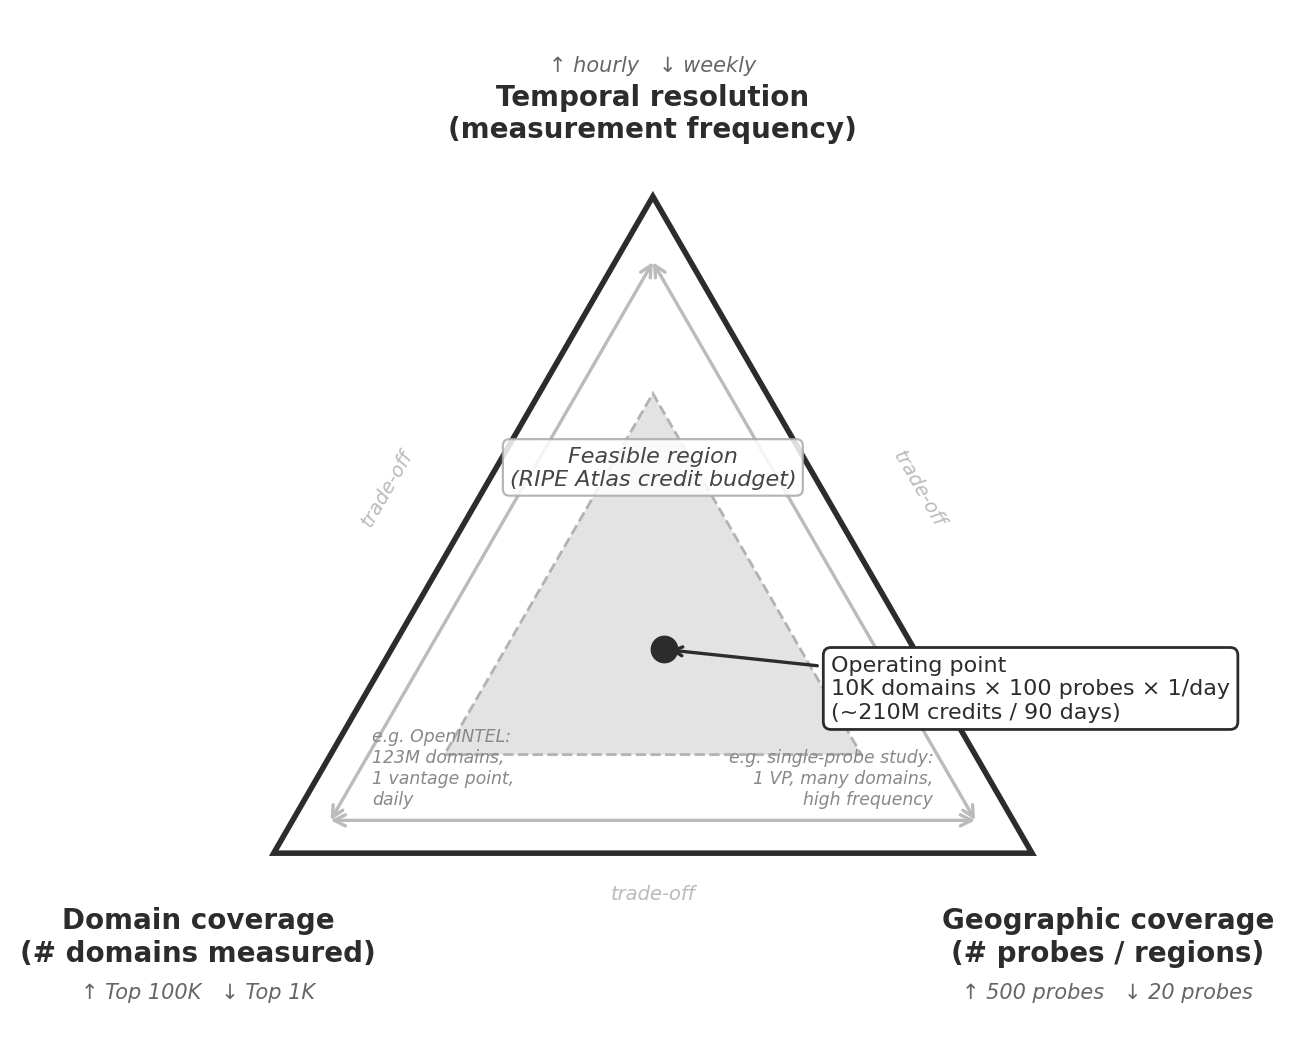
\includegraphics[width=0.62\linewidth]{figures/fig3_constraints_triangle.png}
  \caption{Le triangle de contraintes de mesure à trois dimensions. Toute augmentation de la couverture de domaines, de la couverture géographique ou de la résolution temporelle se fait au détriment des deux autres dimensions, bornée par le budget de crédits RIPE Atlas. Le point de fonctionnement choisi (10\,000 domaines $\times$ 100 sondes $\times$ une fois par jour, $\approx$210M crédits sur 90 jours) est indiqué.}
  \label{fig:constraints_triangle}
\end{figure}

\bigskip
\section{Collecte et traitement des données}
\label{sec:3.4}

\subsection{Pipeline de collecte quotidienne}
\label{subsec:3.4.1}

Les résultats de mesure sont collectés depuis l'API REST RIPE Atlas selon un calendrier quotidien, récupérant les résultats du jour calendaire précédent. Le script de collecte interroge chaque identifiant de mesure actif, récupère tous les résultats dans la fenêtre temporelle spécifiée, et les écrit dans le stockage local en JSON brut. La gestion des erreurs inclut une réessai automatique (trois tentatives avec backoff exponentiel).

\begin{lstlisting}[style=python]
# Pseudocode : collecte quotidienne
def collect_daily(msm_ids, target_date):
    start = target_date.replace(hour=0, minute=0, second=0)
    stop  = target_date.replace(hour=23, minute=59, second=59)
    for msm_id in msm_ids:
        results = atlas_api.get_results(msm_id, start=start, stop=stop)
        write_raw(results, path=f"data/raw/{target_date}/{msm_id}.json")
\end{lstlisting}

\subsection{Analyse syntaxique et extraction des champs}
\label{subsec:3.4.2}

Chaque résultat DNS brut RIPE Atlas est un objet JSON contenant des métadonnées de mesure, des métadonnées de sonde, et la réponse DNS brute (champ \texttt{abuf}, encodé en base64). Le pipeline d'analyse extrait les champs suivants :

\textbf{Métadonnées de mesure} : \texttt{msm\_id}, \texttt{prb\_id}, \texttt{timestamp} (epoch Unix, heure de mesure réelle).

\textbf{Métadonnées de sonde} : \texttt{from} (IP source de la sonde), \texttt{af} (famille d'adresses). Le pays, les coordonnées géographiques et l'ASN de la sonde sont récupérés depuis l'API de métadonnées des sondes RIPE Atlas.

\textbf{Réponse DNS} : Le champ \texttt{abuf} est décodé en base64 et analysé avec la bibliothèque \texttt{dnspython} pour extraire : \texttt{rcode}, \texttt{flags}, \texttt{answer\_records} (liste d'adresses IP avec TTL), \texttt{nsid} (valeur NSID), et \texttt{rt} (temps de réponse en ms).

\subsection{Validation et filtrage des données}
\label{subsec:3.4.3}

Quatre filtres de validation sont appliqués en séquence :

\textbf{Filtre 1 --- Complétude du résultat} : Les résultats sans le champ \texttt{abuf} (aucune réponse DNS reçue dans le délai d'attente) sont classifiés \texttt{TIMEOUT} et exclus de l'analyse de contenu.

\textbf{Filtre 2 --- Validation temporelle} : Les résultats dont l'horodatage réel s'écarte de plus de quatre heures du temps de mesure planifié sont classifiés \texttt{SCHED\_REJECTED}~\cite{Holterbach2015}.

\textbf{Filtre 3 --- Code de réponse DNS} : Les résultats avec \texttt{rcode != NOERROR} sont classifiés par leur code d'erreur spécifique. Pour Q1 et Q2, seuls les résultats \texttt{NOERROR} avec au moins un enregistrement de réponse sont utilisés.

\textbf{Filtre 4 --- Détection de réponse anormale} : Les résultats retournant des adresses IP incohérentes avec l'espace d'adressage connu du domaine interrogé sont signalés. Ce filtre détecte les cas où un proxy en chemin intercepte la requête~\cite{Jones2016}. Le pipeline de validation complet est représenté dans la figure~\ref{fig:pipeline_validation}.

\begin{figure}[tp]
  \centering
  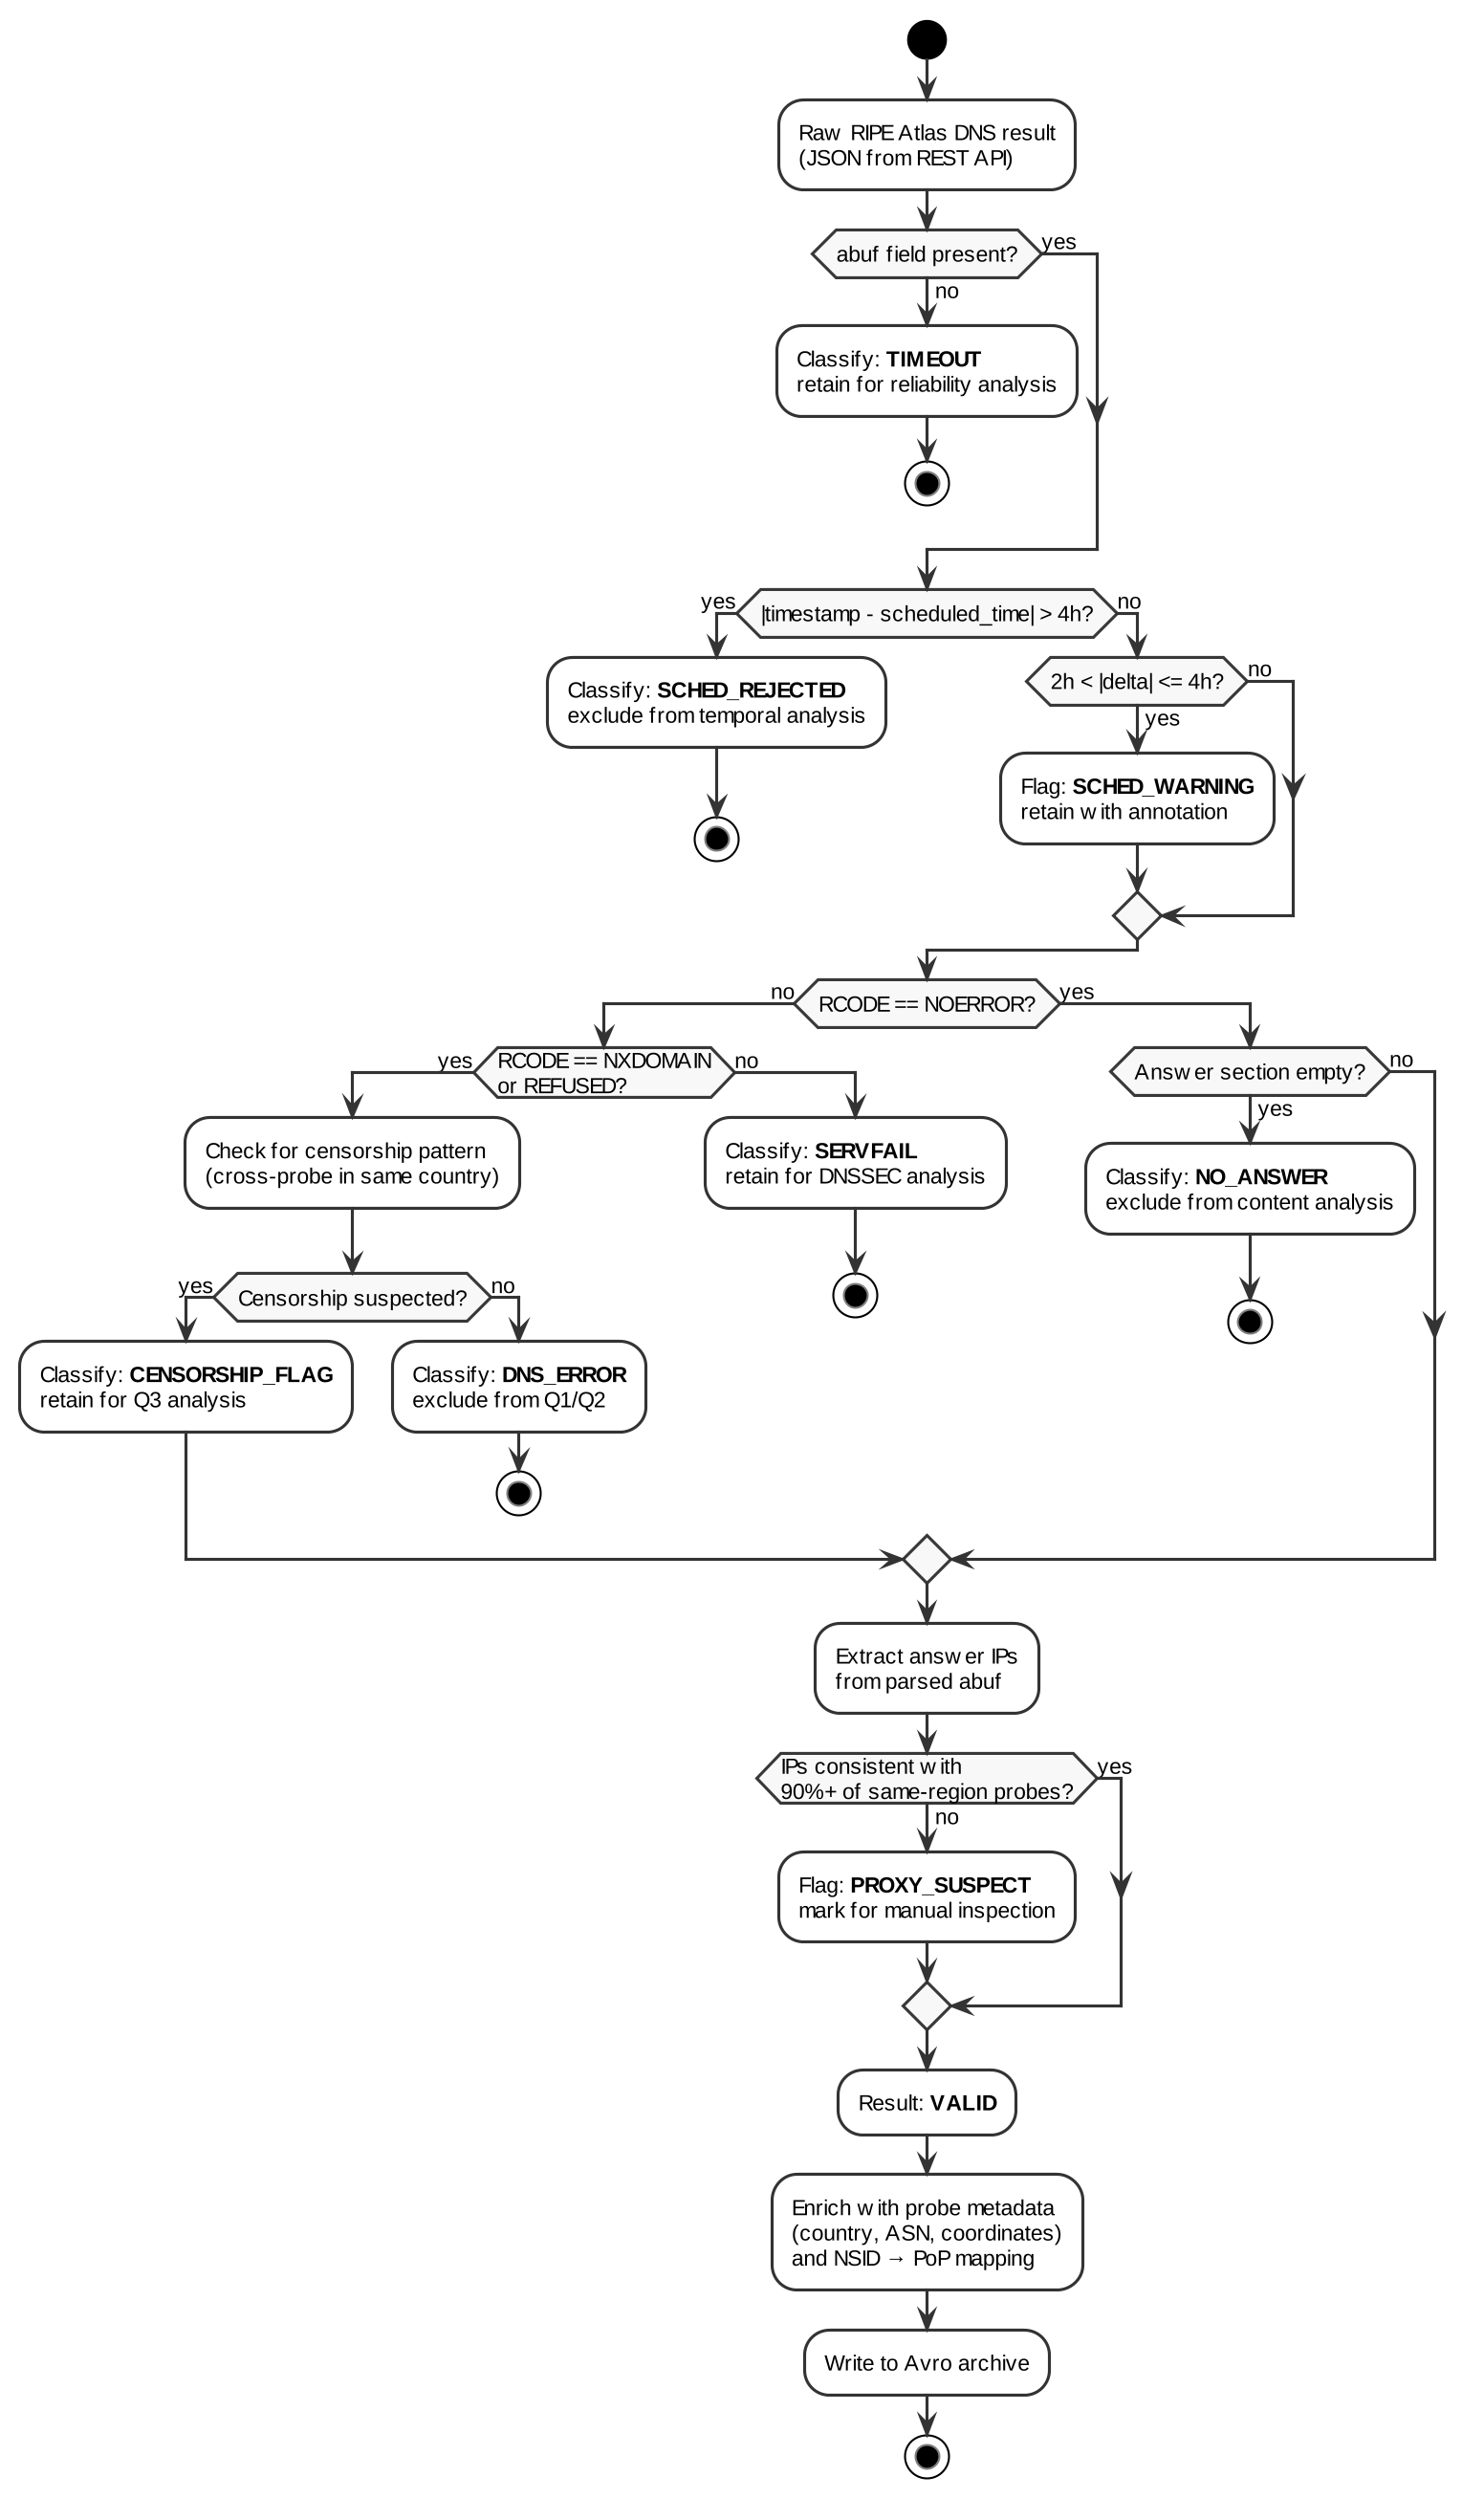
\includegraphics[width=0.72\linewidth]{figures/fig8_pipeline_validation.png}
  \caption{Pipeline de validation et de filtrage des mesures (section~\ref{subsec:3.4.3}). Les quatre filtres séquentiels excluent progressivement les résultats invalides : délais d'attente, déviations de planification, codes d'erreur DNS, et réponses anormales. Seuls les résultats classifiés \texttt{VALID} sont admis dans l'archive Avro.}
  \label{fig:pipeline_validation}
\end{figure}

\begin{table}[H]
\centering
\small
\begin{tabular}{l l l}
\toprule
\textbf{Filtre} & \textbf{Étiquette de classification} & \textbf{Taux d'exclusion attendu} \\
\midrule
Timeout (pas de \texttt{abuf})       & \texttt{TIMEOUT}          & 1--3\,\%             \\
Déviation temporelle $>$4h           & \texttt{SCHED\_REJECTED}  & $\approx$1\,\%       \\
RCODE $\neq$ NOERROR             & \texttt{DNS\_ERROR}       & 2--5\,\%             \\
Réponse anormale (proxy)  & \texttt{PROXY\_SUSPECT}   & $<$1\,\%             \\
\midrule
\textbf{Résultats utilisables (VALID)}  &                           & \textbf{$\approx$90--95\,\%} \\
\bottomrule
\end{tabular}
\caption{Taux d'exclusion attendus par filtre de validation~\cite{Holterbach2015,Jones2016,Nosyk2024}.}
\label{tab:filter_rates}
\end{table}

\subsection{Enrichissement des métadonnées}
\label{subsec:3.4.4}

Les métadonnées de sondes (coordonnées géographiques, pays, ASN) sont enrichies depuis deux sources : l'API de métadonnées des sondes RIPE Atlas (source primaire) et la base de données MaxMind GeoLite2 City (validation croisée secondaire). Jones et al.~\cite{Jones2016} notent que 1,7\,\% des sondes RIPE Atlas ont une géolocalisation incohérente entre les deux sources.

Les chaînes NSID des serveurs faisant autorité sont mappées à des emplacements PoP physiques en utilisant les conventions de nommage décrites par Bortzmeyer~\cite{Bortzmeyer2013} et Finnegan~\cite{Finnegan2018} : codes IATA aéroportuaires (ex. \texttt{ams} $\rightarrow$ Amsterdam Schiphol, \texttt{fra} $\rightarrow$ Francfort) et abréviations de villes.

\subsection{Architecture de stockage}
\label{subsec:3.4.5}

Les résultats sont stockés dans une architecture à deux niveaux suivant la conception d'OpenINTEL~\cite{vanRijswijk2016} :

\textbf{Niveau 1 --- Archivage long terme (Apache Avro)} : Les résultats analysés sont sérialisés au format Apache Avro. L'encodage binaire d'Avro avec compression snappy atteint un taux de compression d'environ 7:1 par rapport au JSON brut~\cite{vanRijswijk2016}, réduisant le stockage quotidien d'environ 2 Go (JSON brut) à environ 280 Mo. Le schéma Avro est présenté dans le tableau~\ref{tab:avro_schema}.

\begin{table}[H]
\centering
\small
\begin{tabularx}{\linewidth}{p{3.2cm} p{2.4cm} X}
\toprule
\textbf{Champ} & \textbf{Type} & \textbf{Description} \\
\midrule
\texttt{msm\_id}          & \texttt{long}          & ID de mesure RIPE Atlas \\
\texttt{prb\_id}          & \texttt{long}          & ID de sonde RIPE Atlas \\
\texttt{timestamp}        & \texttt{long}          & Heure de mesure réelle (epoch Unix) \\
\texttt{domain}           & \texttt{string}        & Nom de domaine interrogé \\
\texttt{query\_type}      & \texttt{string}        & \texttt{A}, \texttt{AAAA}, ou \texttt{NS} \\
\texttt{campaign\_type}   & \texttt{string}        & \texttt{auth\_direct} | \texttt{isp\_resolver} | \texttt{public\_dns} | \texttt{public\_dns\_noecs} \\
\texttt{probe\_country}   & \texttt{string}        & Code pays ISO 3166-1 alpha-2 \\
\texttt{probe\_asn}       & \texttt{long}          & Numéro de système autonome \\
\texttt{probe\_lat/lon}   & \texttt{double}        & Coordonnées géographiques de la sonde \\
\texttt{rcode}            & \texttt{int}           & Code de réponse DNS (NOERROR=0, NXDOMAIN=3, SERVFAIL=2\ldots) \\
\texttt{answer\_ips}      & \texttt{array[string]} & Enregistrements A/AAAA retournés \\
\texttt{answer\_ttl}      & \texttt{long}          & TTL des enregistrements de réponse (secondes) \\
\texttt{nsid}             & \texttt{string}        & Valeur de l'option NSID ; chaîne vide si absente \\
\texttt{rt\_ms}           & \texttt{double}        & Temps de réponse en millisecondes \\
\texttt{valid}            & \texttt{boolean}       & \texttt{true} si le résultat passe les quatre filtres \\
\texttt{validation\_flag} & \texttt{string}        & \texttt{VALID} | \texttt{TIMEOUT} | \texttt{SCHED\_REJECTED} | \texttt{DNS\_ERROR} | \texttt{PROXY\_SUSPECT} \\
\bottomrule
\end{tabularx}
\caption{Schéma Apache Avro pour les enregistrements de mesure DNS. Chaque ligne correspond à un résultat de requête DNS d'une sonde RIPE Atlas.}
\label{tab:avro_schema}
\end{table}

\textbf{Niveau 2 --- Analytique (Apache Parquet)} : Les enregistrements Avro validés sont convertis quotidiennement au format Apache Parquet, partitionnés par année/mois/jour. Le format de stockage en colonnes de Parquet permet l'exécution efficace des requêtes analytiques sans lire tous les champs.

\textbf{Estimation de stockage} : Pour la campagne principale, le stockage total requis est d'environ :
\begin{itemize}
  \item JSON brut : $\sim$180 Go
  \item Avro : $\sim$24 Go
  \item Parquet : $\sim$18 Go
  \item \textbf{Total : $\sim$220 Go} (archive long terme $\sim$42 Go)
\end{itemize}

\bigskip
\section{Méthodes d'analyse}
\label{sec:3.5}

\subsection{Q1 --- Diversité géographique des réponses DNS}
\label{subsec:3.5.1}

\textbf{Objectif} : Pour chaque domaine du corpus, déterminer si l'ensemble des adresses IP retournées varie systématiquement selon la localisation géographique de la sonde qui interroge.

\textbf{Étape 1 --- Calcul de la diversité IP par domaine} : Pour chaque domaine et chaque jour de mesure, l'ensemble des adresses IP uniques retournées par toutes les sondes est calculé. Le \textbf{nombre d'adresses IP distinctes} observées fournit un premier indice de diversité.

\textbf{Étape 2 --- Calcul de la diversité inter-régions} : Pour chaque domaine, l'ensemble de sondes est partitionné par région géographique. Pour chaque paire de régions, la similarité de Jaccard entre leurs ensembles d'adresses IP est calculée :

\[
J(A, B) = \frac{|A \cap B|}{|A \cup B|}
\]

Une similarité de Jaccard de 1,0 indique des ensembles IP identiques (pas de différenciation géographique) ; 0 indique des ensembles entièrement disjoints (différenciation géographique complète). La \textbf{similarité de Jaccard médiane par paires} entre toutes les paires de régions sert de métrique primaire de diversité géographique par domaine.

\textbf{Étape 3 --- Classification} : Les domaines sont classifiés en quatre catégories de diversité géographique :

\begin{table}[H]
\centering
\small
\begin{tabular}{l l l}
\toprule
\textbf{Catégorie} & \textbf{Critère} & \textbf{Interprétation} \\
\midrule
\texttt{UNIFORM} & Une seule IP pour toutes les sondes & Pas de routage géographique \\
\texttt{LOW\_DIVERSITY} & Jaccard médian > 0,8 & Variation minimale (round-robin) \\
\texttt{MEDIUM\_DIVERSITY} & Jaccard médian 0,4--0,8 & Routage géographique modéré \\
\texttt{HIGH\_DIVERSITY} & Jaccard médian < 0,4 & Routage géographique fort \\
\bottomrule
\end{tabular}
\end{table}

\textbf{Étape 4 --- Attribution du mécanisme} : Pour les domaines de la catégorie \texttt{HIGH\_DIVERSITY}, les chaînes NSID retournées par le serveur faisant autorité permettent de déterminer si la variation géographique est due à la sélection d'instance anycast (NSID différent par région) ou au routage CDN DNS (même NSID mais adresses IP différentes).

\subsection{Q2 --- Stabilité temporelle}
\label{subsec:3.5.2}

\textbf{Objectif} : Quantifier la stabilité temporelle des réponses DNS pour chaque domaine.

\textbf{Méthode} : Pour chaque domaine et chaque sonde, la série temporelle des ensembles d'adresses IP est extraite. Les observations journalières consécutives sont comparées par similarité de Jaccard. L'indice de stabilité quotidienne au niveau du domaine est la médiane des indices de stabilité de sondes. L'analyse est répétée aux échelles hebdomadaire et mensuelle. La corrélation de Spearman entre le TTL médian des enregistrements A et le taux de changement quotidien teste l'hypothèse que les domaines avec des TTL courts présentent des changements plus fréquents.

\subsection{Q3 --- Évaluation du biais géographique de RIPE Atlas}
\label{subsec:3.5.3}

\textbf{Méthode} : L'évaluation du biais géographique utilise une \textbf{expérience de sous-échantillonnage contrôlée}. Trois ensembles virtuels de sondes sont construits :

\begin{enumerate}
  \item \textbf{ACTUAL} : L'ensemble de sondes déployé complet.
  \item \textbf{EUROPE\_NA\_ONLY} : Uniquement les sondes en Europe et en Amérique du Nord.
  \item \textbf{UNIFORM} : Un ensemble rééchantillonné avec un nombre égal de sondes par continent.
\end{enumerate}

La métrique de diversité géographique est recalculée pour chaque ensemble virtuel de sondes. Les distributions sont comparées avec le test de Wilcoxon des rangs signés (test non paramétrique par paires). La \textbf{contribution unique en IP} de chaque région est calculée : la fraction des adresses IP observées uniquement depuis les sondes d'une région spécifique.

\subsection{Q4 --- Impact du choix de résolveur}
\label{subsec:3.5.4}

\textbf{Méthode} : Cette analyse utilise la campagne supplémentaire Q4 qui fournit quatre observations simultanées pour les 1\,000 domaines Tranco Top depuis le même ensemble de sondes :

\begin{enumerate}
  \item \texttt{auth\_direct} : Requête directe au serveur faisant autorité
  \item \texttt{isp\_resolver} : Résolveur ISP local
  \item \texttt{public\_dns} : Google Public DNS (8.8.8.8)
  \item \texttt{public\_dns\_noecs} : Google Public DNS avec opt-out ECS
\end{enumerate}

Pour chaque domaine et chaque sonde, les quatre ensembles d'adresses IP sont comparés par similarité de Jaccard. Les comparaisons sont désagrégées par continent. Le test de Mann-Whitney U (non paramétrique, avec correction de Bonferroni pour six comparaisons) valide statistiquement les différences.

\bigskip
\section{Considérations éthiques et reproductibilité}
\label{sec:3.6}

\subsection{Conception éthique}
\label{subsec:3.6.1}

La conception de la mesure suit le cadre éthique de Kisteleki et al.~\cite{Kisteleki2016} :

\textbf{Protection des hôtes de sondes} : Toutes les cibles interrogées sont des domaines publiquement accessibles du corpus Tranco Top 10K. Aucun domaine politiquement sensible ou à restriction juridictionnelle n'est inclus.

\textbf{Impact sur l'infrastructure} : La fréquence de mesure (une fois par domaine par jour) est des ordres de grandeur en dessous du seuil qui constituerait une charge excessive sur les serveurs DNS faisant autorité~\cite{vanRijswijk2016}. Cette campagne génère environ un million de requêtes par jour --- environ 1\,000 fois moins qu'OpenINTEL.

\textbf{Transparence} : Toutes les mesures sont étiquetées \texttt{thesis-dns-geo} dans RIPE Atlas.

\textbf{Minimisation des données} : Les résultats bruts incluent les adresses IP des sondes, qui ne sont pas publiées. Le jeu de données public utilise uniquement des statistiques agrégées par pays et par ASN.

\subsection{Reproductibilité scientifique}
\label{subsec:3.6.2}

\textbf{Corpus de domaines fixe} : L'identifiant de liste Tranco utilisé chaque semaine de mesure est enregistré dans les métadonnées du jeu de données.

\textbf{Traçabilité des mesures} : Tous les identifiants de mesure RIPE Atlas sont enregistrés dans le manifeste du jeu de données.

\textbf{Publication du jeu de données} : Le jeu de données final (format Avro + Parquet) est publié sur Zenodo avec un DOI permanent avant la défense orale, suivant les principes FAIR~\cite{vanRijswijk2016}.

\textbf{Validation pilote} : Avant la campagne de production de trois mois, une campagne pilote de sept jours sur un sous-ensemble de 500 domaines avec 10 sondes valide la configuration de mesure et estime la consommation réelle de crédits.
\bigskip
